\subsection{Timeedit}
I det följande avsnittet kommer TekNat-fakultetens instans av
planeringsverktyget Timeedit att kallas för tjänsten. Den modul i tekweb
vid namn timeedit som arbetar mot tjänsten kommer att kallas för
modulen.

\subsubsection{Bakgrund}
Text som beskriver bakgrunden till modulen

\subsubsection{Mål}
Modulens syfte är att tillgängliggöra den funktionalitet som är synlig
mot studenterna hos tjänsten. Modulen skapades eftersom projektgruppen
och beställaren tidigt var överens om att de tänkta användarna skulle
betrakta funktionaliteten som en kärnfunktion.

\subsubsection{Begränsningar}
Här skriver vi om de medvetna begränsningar som gjordes av modulen
p.g.a. tidsbegränsningar, svåra tekniska problem, buggar, m.m.

\subsubsection{Informationsflöde}
Att beskriva modulen i sitt sammanhang samt den hjälpklass som används
(LibTimeEdit) görs bäst genom att först visa informationsflödet med
hjälp av följande bild och sedan sätta ord kring det som visas i bilden
nedan.

Beskriv saker som modulen gör, relatera dem till bilden.

\begin{wrapfigure}{r}{0.5\textwidth}
  \begin{center}
    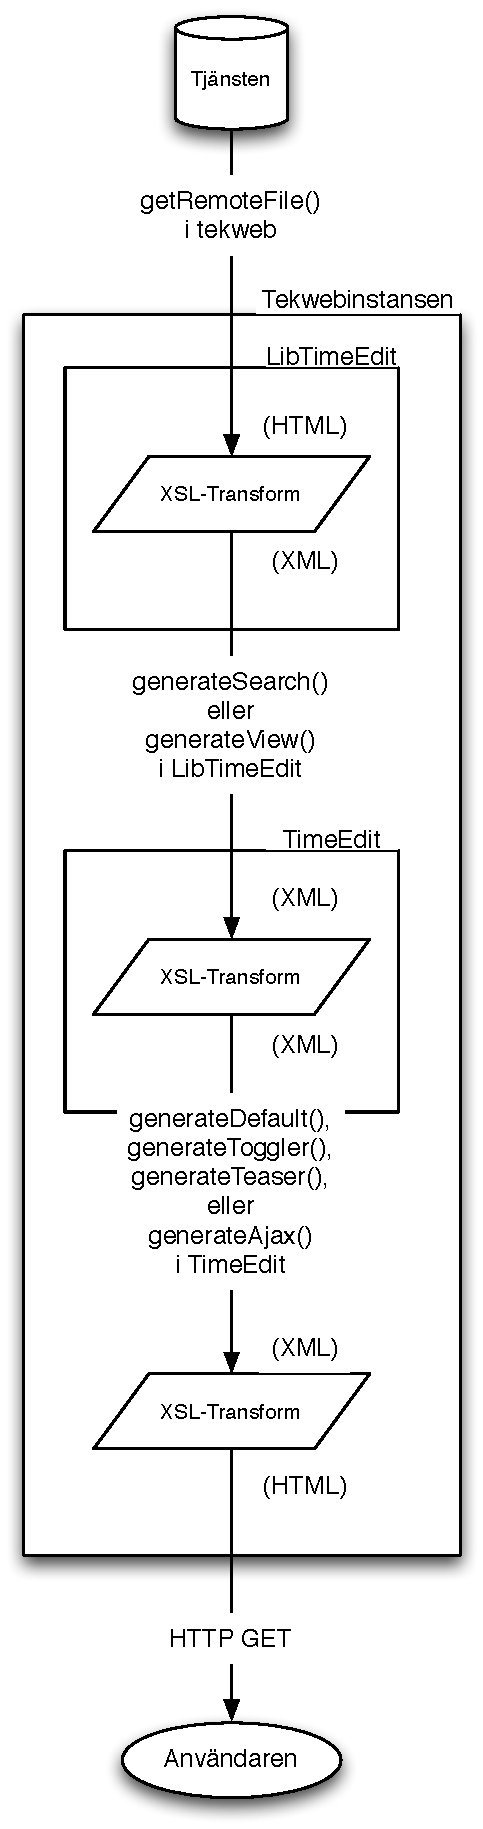
\includegraphics[width=45mm]{timeeditchart.pdf}
  \end{center}
  \caption{TimeEdit i sitt sammanhang.}
\end{wrapfigure}

